\chapter{Evaluation und Vergleich zu anderen Lösungsansätzen}
\label{chapter:vgl}

Bei der Entwicklung unserer Lösung sind noch andere Ansätze entstanden, welche nach Evaluation mit unserem Ansatz aus Kapitel \ref{chapter:algo}, aber nicht weiter ausgearbeitet oder ausgewertet wurden. Für die Vollständigkeit stellen wir nun noch kurz einen alternativen kräftebasierten Ansatz (\ref{UniformK-Ansatz}) und einen hierarchischen Ansatz (\ref{Hierarch-Ansatz}) vor. Ein kurzer Vergleich wird in Abschnitt \ref{Ansatz-Vergleich} gezeigt.

\section{Uniform kräftebasiertes Layout}
\label{UniformK-Ansatz}
Dieser Lösungsansatz stellt eine einfache Erweiterung zu vorhandenen kräftebasierten Algorithmen dar: Knoten können durch zusammenfassende Pseudoknoten repräsentiert werden, wie sie bereits in \cite{gdea_3362} für Berechnungsapproximationen verwendet wurden, und es werden zusätzlich \glqq Anker\grqq\ verwendet.

Konkret bedeutet dies, dass Knoten zunächst nur durch ihre zusammengefassten Pseudoknoten darstellt werden und hierfür mit einem einfachen kräftebasierten Verfahren ein Layout bestimmen, wobei die abstoßende Kraft der Pseudoknoten bzw. die Anziehungskraft zusammengelegter Kanten logarithmisch mit der Anzahl zusammengefassten Elemente skaliert wird.
%Würde das mit logarithmischen Kräften/Größen schon stehen lassen, sonst müssen wir den ganzen Text ändern um weg von Pseudoknoten und hin zu geschlossenen Gruppen zu gehen.

Wenn nun die Elemente einer oder mehrerer Gruppen konkret dargestellt werden sollen, so werden die Pseudoknoten zunächst ähnlich wie bei der finalen Lösung verankert. Zusätzlich werden die Pseudoknoten deren Elemente dargestellt werden sollen aus dem Layout entfernt und stattdessen die Knoten der Gruppe, die ebenfalls Pseudoknoten für innere Gruppen sein können, eingefügt. Schließlich wird nun noch einmal der kräftebasierte Algorithmus verwendet mit der Besonderheit, dass jeder Knoten eine zusätzliche Anziehung zu seinem Anker bzw. dem Anker des übergeordneten Pseudoknotens.

Dieser Ablauf wird in Abbildung \ref{UniformK-Skizze} skizziert.

\begin{figure}[h!]
\begin{center}
	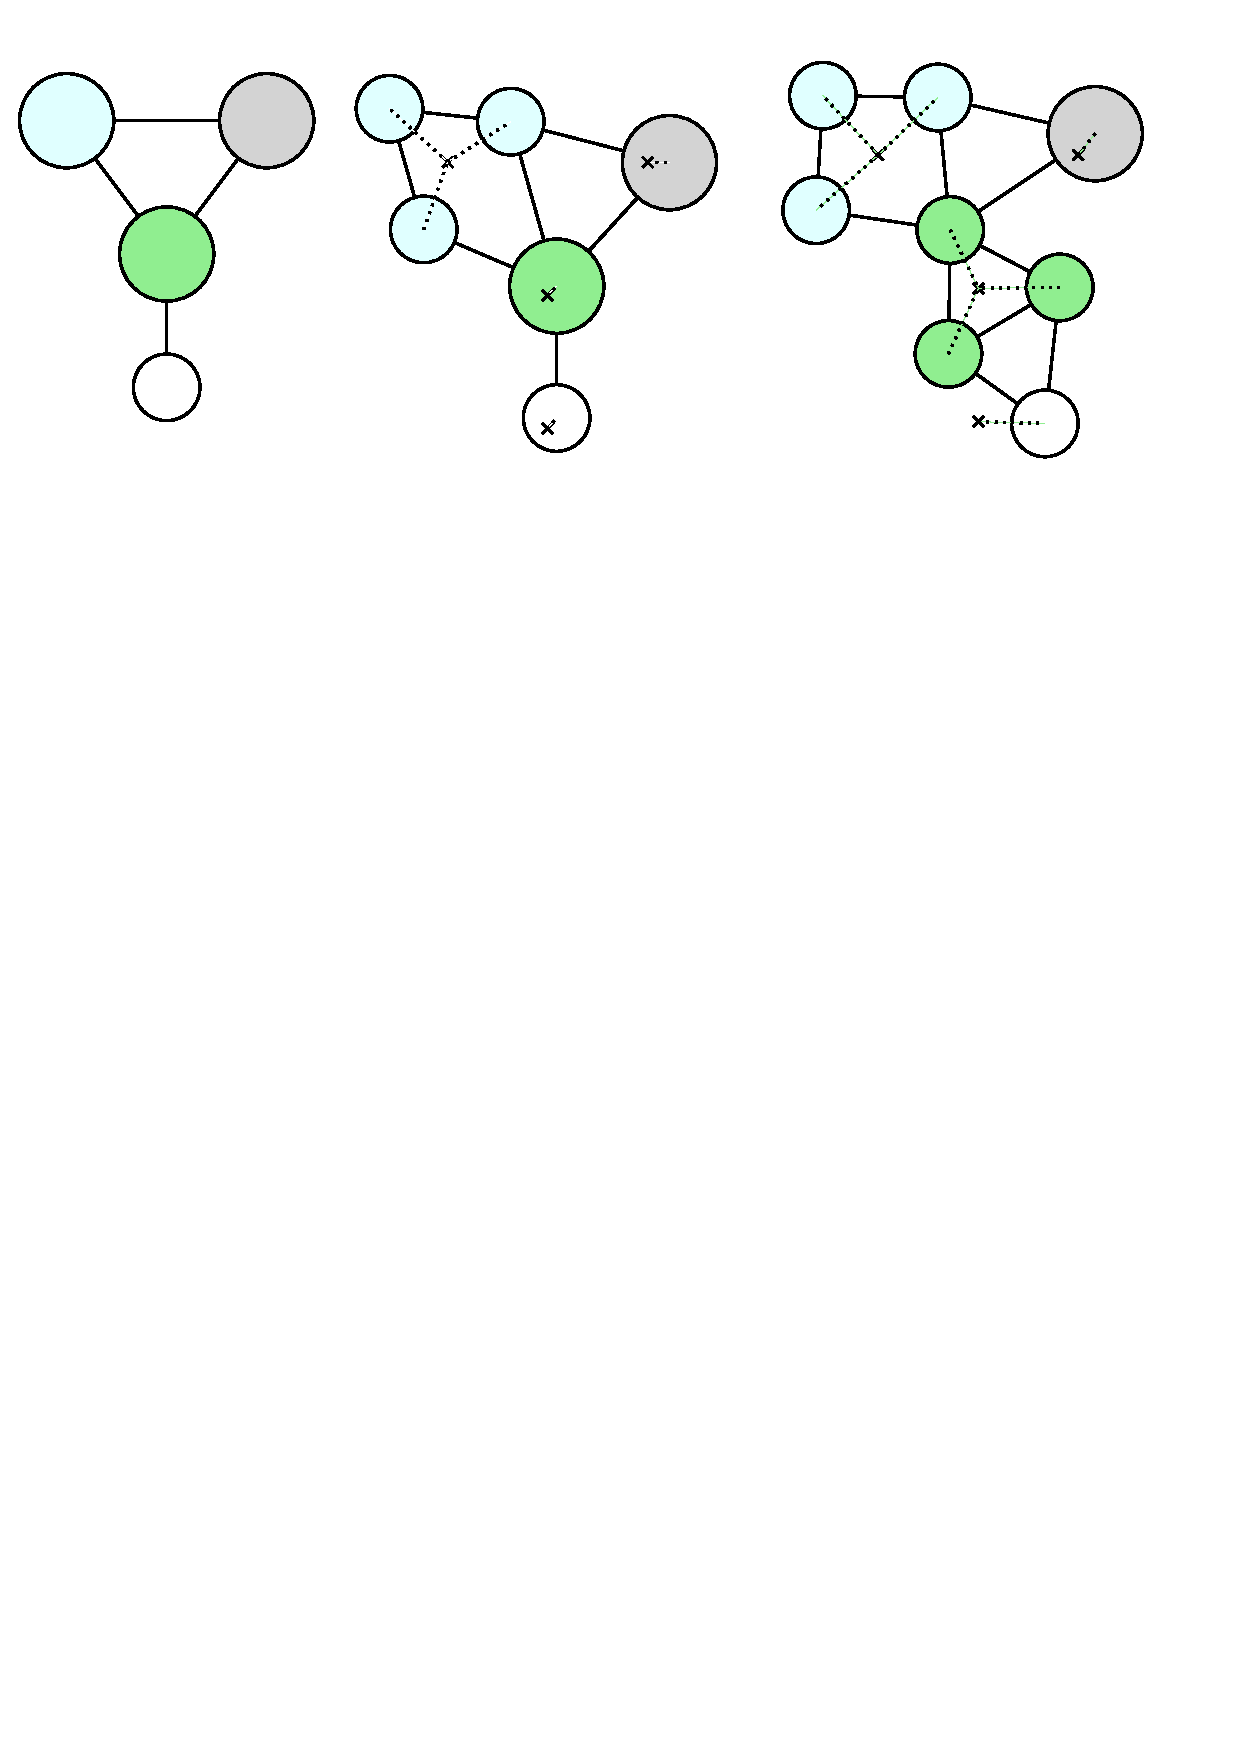
\includegraphics[width=\textwidth]{Pics/uniform_kb.pdf}
	\caption{Skizze eines Layouts durch den uniform krqftebasierten Ansatz. Links zunächst das Layout mit alle Gruppen geschlossen. In der Mitte das Layout nach Öffnen der hellblauen Gruppe. Rechts das Layout mit hellblauer und grüner Gruppe geöffnet. Kreuze markieren hierbei die Anker der Gruppen.}
	\label{UniformK-Skizze}
\end{center}
\end{figure}

% zu vergleichen mit hierarchischem Layout und alles kräftebasiert

\section{Hierarchisches Layout}
\label{Hierarch-Ansatz}
Häufig auftretende Eigenschaften in Argumentkarten wie Zyklenfreiheit legen andere Graphenlayouts, insbesondere hierarchische Layouts, nahe.

Wenn wir die Richtung der Kanten, entgegen der bisherigen Ansätze, für das Layout beachten wollen, wird es dadurch möglich bei einem hierarchischen Layout alle eingehenden Kanten eines Knotens an der Oberseite des Knotens und alle ausgehenden Kanten an der Unterseite des Knotens zu zeichnen. Dadurch wird ebenfalls das \glqq einpacken \grqq\ der Knoten in eine Box zur Repräsentation bzw. Ordnung der Gruppe einfacher, da auch die Box der Gruppe die ein- und ausgehenden Kanten entsprechend ordnen kann ohne die Komplexität des Layouts innerhalb der Box zu erhöhen, wodurch das innere und äußere Layout von Gruppen getrennt berechnen werden können.

Ein grobe Skizze zu einem solchen Layout ist in Abbildung \ref{Hierarch-Skizze} dargestellt.

\begin{figure}[h!]
\begin{center}
	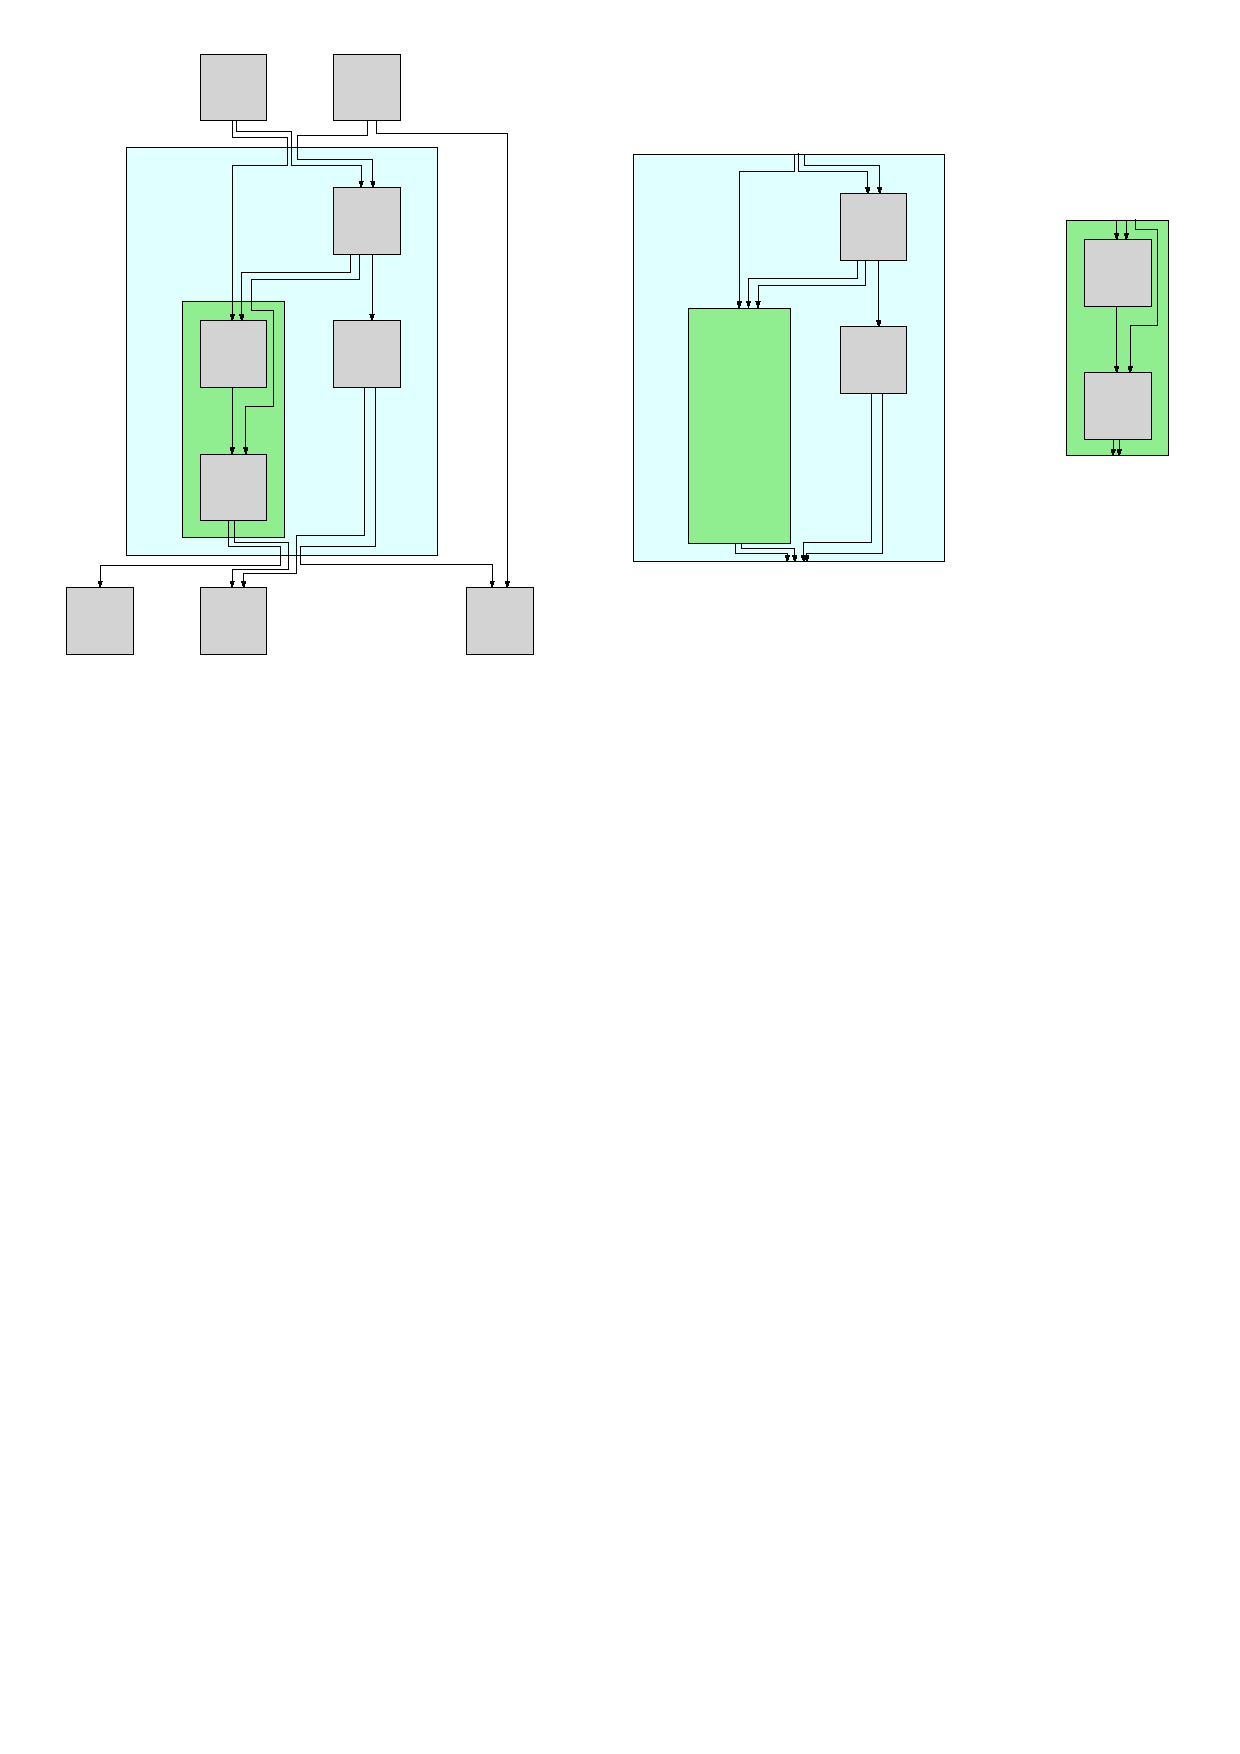
\includegraphics[width=\textwidth]{Pics/hierarchisch.pdf}
	\caption{Skizze eines Layouts durch den hierarchischen Ansatz. Links das Gesamtlayout, Mitte und Rechts jeweils das Layout der jeweiligen Gruppe.}
	\label{Hierarch-Skizze}
\end{center}
\end{figure}

\section{Vergleich}
\label{Ansatz-Vergleich}
Da keiner der Ansätze konkret implementiert wurde und die alternativen Ansätze auch stückweise ausgearbeitet wurden, besteht der Vergleich dieser Ansätze größtenteils aus Abschätzungen und nicht tatsächlichen Messungen. Es werden folgende Abkürzungen verwendet:

\textbf{KBK}: Unser Lösungsansatz, der kräftebasierte Algorithmus mit Kapselung

\textbf{HL}: Der hierarchische Layout-Ansatz

\textbf{UKB}: Der uniform kräftebasierte Layout-Algorithmus

\paragraph*{Fokus des Layouts}
Bei KBK und HL sind die Layouts der einzelnen Gruppenebenen größtenteils unabhängig, daher liegt der Fokus der Darstellung eher auf der Semantik der Gruppen, d.h. das Layout stellt besonders heraus, zu welcher Gruppe ein Knoten gehört.

Das durch UKB erzeugte Layout basiert dagegen größtenteils auf den Knotenzusammenhängen ab. Durch die Anker bleiben Gruppenelemente zwar größtenteils zusammen, aber das Layout wird dennoch über die Kanten der Knoten in und zwischen Gruppen festgelegt. Bei entsprechenden Zusammenhängen können Gruppen auch deformiert oder getrennt werden (siehe Abbildung \ref{Uniform-Trenn-Skizze}).

\begin{figure}[h]
\begin{center}
	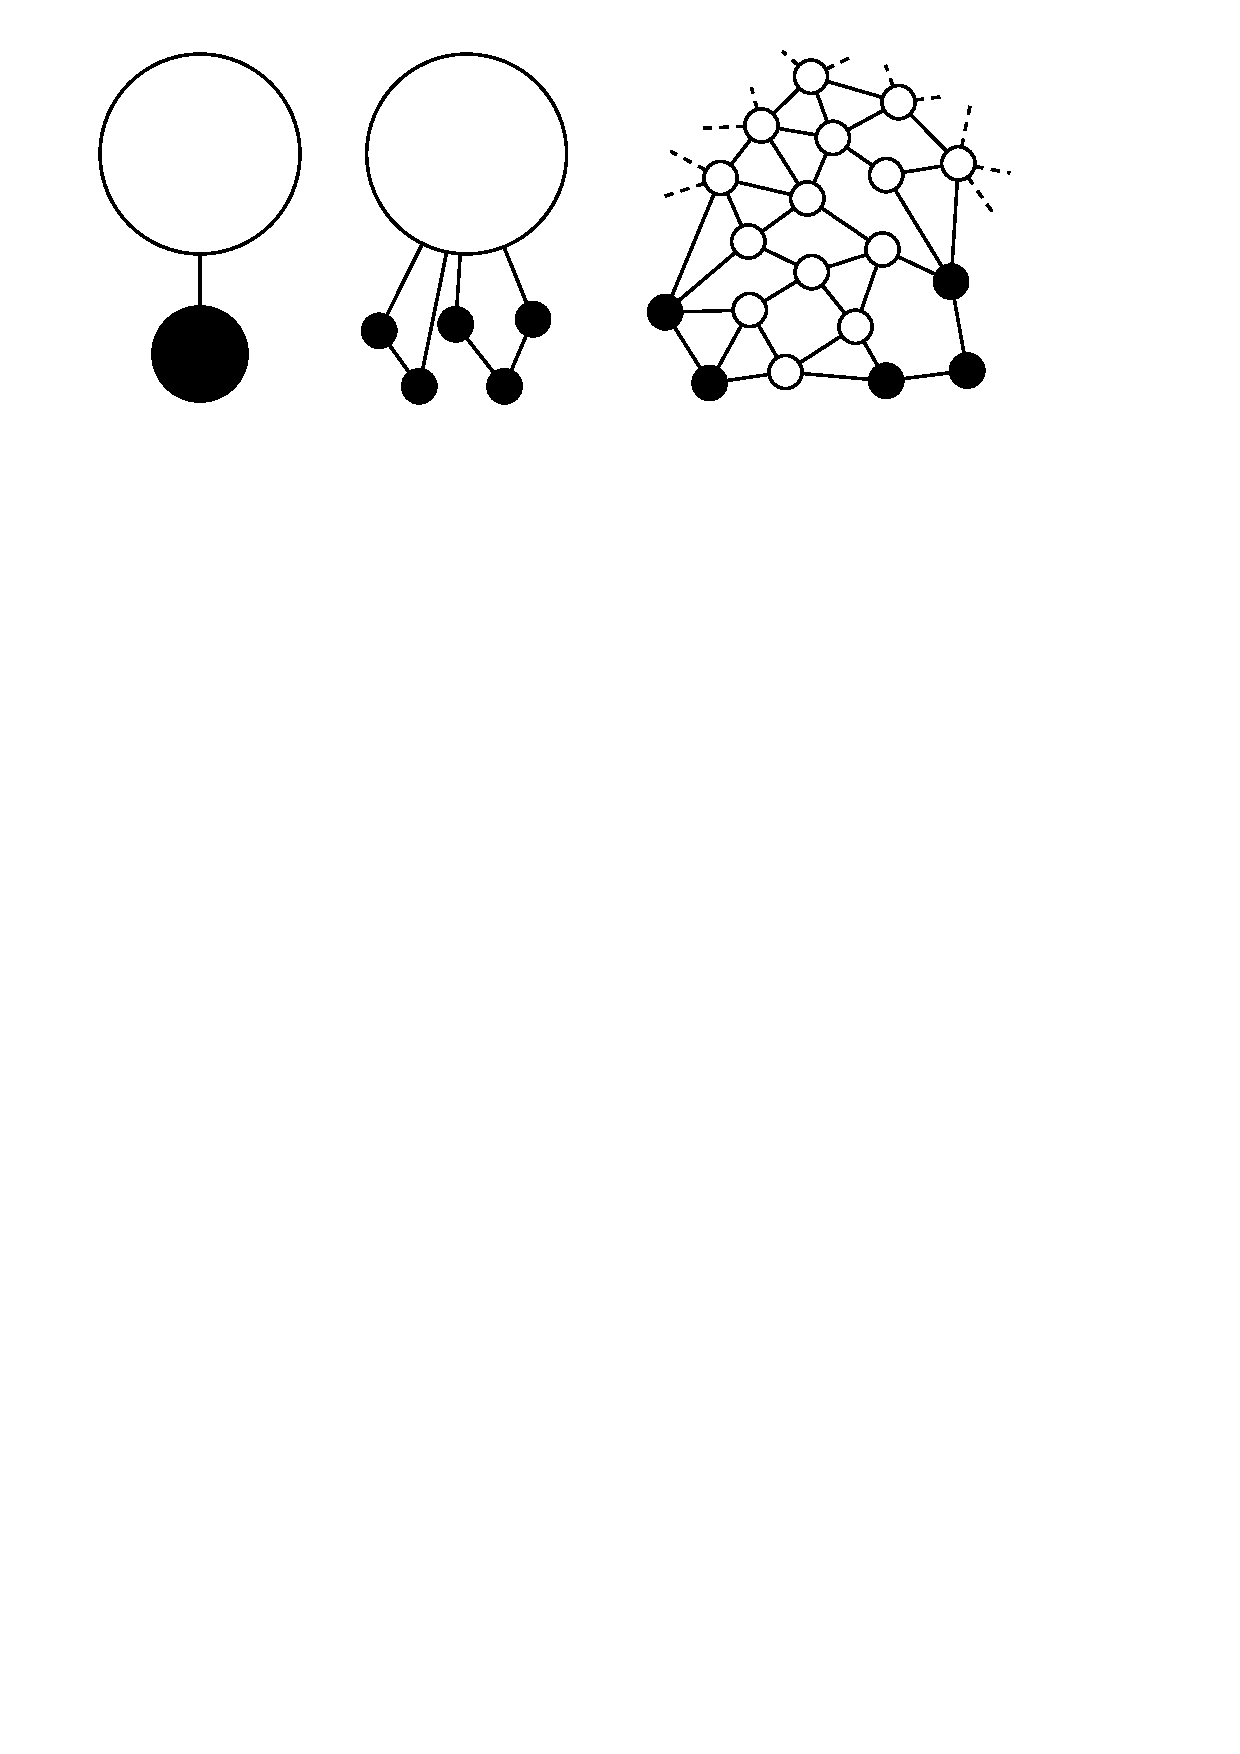
\includegraphics[width=\textwidth]{Pics/uniform_trenn.pdf}
	\caption{Beispielhafter Ablauf der zur Trennung einer Gruppe führt: Durch ungünstige Kantenzusammenhänge und einen entscheidenden Größenunterschied drängt sich die weiße Gruppe zwischen die Knoten der schwarzen Gruppe.}
	\label{Uniform-Trenn-Skizze}
\end{center}
\end{figure}


\paragraph*{Änderungskonstanz}
Durch die unabhängigen internen und externen Gruppenlayouts bei KBK und HL, sind die Änderungen beim Öffnen und Schließen von Gruppen eher gering: Die Layouts in den Gruppen ist unabhängig davon ob andere Gruppen geöffnet oder geschlossen sind und die relativen Positionen der Gruppen zueinander ändern sich selten.

Da bei UKB die Gruppen nicht \glqq geschirmt \grqq\ sind, ist das Layout geöffneter Gruppen sehr stark vom Zustand anderer Gruppen abhängig. Die relativen Positionen bleiben durch die Anker zwar meist erhalten, aber kleine Gruppen sind durchaus anfällig von großen Gruppen deformiert bzw. verdrängt zu werden.

\paragraph*{Komplexität des Algorithmus}
Wie bereits in Kapitel 3 dargestellt, ist der für KBK nötige Algorithmus recht komplex und enthält einige Parameter, die noch bestimmt werden müssen.

Der für HL benötigt Algorithmus benötigt etwas weniger Komplexität als KBK, da die Port für Kanten stets fest sind, wodurch die Größe von geöffneten Gruppen einmalig \glqq Bottom-Up \grqq\ bestimmt werden kann ohne Approximationen und Korrekturen. Allerdings besitzt der zugrundeliegende Algorithmus für hierarchisches Layouts eine höhere Komplexität als kräftebasierende Verfahren.

Der UKB-Algorithmus stellt schließlich eine algorithmisch weniger komplexe Erweiterung von einfachen kräftebasierten Verfahren dar, was vermutlich zu der geringsten Komplexität unter den hier verglichenen Ansätzen führt.

\paragraph*{Anforderung an Graphen}
Während alle hier vorgestellten Ansätze davon ausgehen, dass jeder Knoten und jede Gruppe maximal einer übergeordneten Gruppe zugehört, werden nur bei HL tatsächliche Anforderungen an die eigentliche Graphenstruktur (Zyklenfreiheit) gestellt um problemlos zu funktionieren.

\paragraph*{Kompaktheit}
Sowohl bei KBK als auch bei HL verliert man durch die Kapselung von Gruppen viel Kompaktheit, da hierbei oft Räume in den Gruppen entstehen, die nicht von anderen Gruppen und Knoten genutzt werden können. Das Gesamtlayout bei KBK ist allerdings bei allen Graphen eher zentriert und rund, da es kräftebasiert bestimmt wird, während HL bei unausgeglichenen Graphen zu besonders hohen bzw. stellenweise sehr breiten Graphen führt.

Das Layout des UKB-Ansatzes führt zu ähnlich kompakten Graphen wie herkömmliche kräftebasierte Algorithmen, da die einzigen zusätzlichen Kräfte, die Anker, an den Positionen der Gruppenknoten gesetzt werden, also in der Hüllkurve des Graphen liegen, und ausschließlich anziehend wirken.

\section*{Fazit}
Wie man an den Einzelpunkten erkennt, vereint der Ansatz für den wir uns entschieden haben viele der positiven Eigenschaften der beiden anderen Ansätze bzw. stellt einen Kompromiss zwischen den beiden dar.
\todo[inline]{Allgemeine Auswertung des Ansatzes/Verfahren schreiben?}
% gesammelte Argumente
	% KB alles kräftebasiert, HS hierarchisch/''Stufen''-Layout
% + Gruppen vorallem semantisch organisiert, weniger strukturell als bei KB
% + Änderungskonstanz der Gruppen (innerhalb von Gruppe) als bei KB
% - komplexer als KB
% + Gruppen überschneiden sich nicht wie bzw einfach zu getrennt zu halten als bei KB 
% + HS ist nur ohne Zykel gut umsetzbar
% + komptakter als HS
% - Struktur evtl nicht so sichtbar wie bei HS aber auch wie bei KB
% + iterativ anwendbar
% + schöner :)
% o Gruppen im Vordergrund der Darstellung durch Ports, nicht Knoten
% o Kantenrounting nicht unbedingt trivial
% 
